% !TEX root = ../om_ts_04.tex

\begin{frame} % название фрагмента

\videotitle{Частные корреляции}

\end{frame}



\begin{frame}{Частные корреляции: план}
  \begin{itemize}[<+->]
    \item Проекция для случайных величин. 
    \item Общее определение. 
    \item Частная автокорреляционная функция. 
  \end{itemize}

\end{frame}


\begin{frame}
  \frametitle{Геометрия случайных величин}

  \begin{block}{Длина и угол}
    Дисперсия $\Var(R)$ — \alert{квадрат длины} случайной величины.

    Корреляция $\Corr(L, R)$ — \alert{косинус угла} между случайными величинами.
  \end{block}
  \pause
  \begin{block}{Ортогональность}
  Величины $L$ и $R$ \alert{ортогональны}, если $\Cov(L, R) = 0$.     
  \end{block}

\end{frame}

\begin{frame}
  \frametitle{Проекция}

  \begin{block}{Обозначение}
    $Best(L; R_1, R_2, \ldots R_n)$ — линейная комбинация 1 и $R_1$, \ldots, $R_n$, 
    \alert{наиболее} похожая на $L$.
  \end{block}
  \pause
  $\hat L = Best(L; R_1, R_2, \ldots R_n)$ если:
  \begin{itemize}[<+->]
    \item $\hat L = \alpha_0 \cdot 1 + \alpha_1 R_1 + \ldots + \alpha_n R_n$;
    \item Ожидание $\E((L - \hat L)^2)$ минимально. 
  \end{itemize}  
\end{frame}


\begin{frame}
  \frametitle{Как найти проекцию?}

  Хотим найти $\hat L = Best(L; R_1, R_2, \ldots R_n)$:
  \[
    \hat L = \alpha_0 \cdot 1 + \alpha_1 R_1 + \ldots + \alpha_n R_n.
  \]

  Как найти коэффициенты?
  \pause
  
  \begin{itemize}[<+->]
    \item Минимизация:
  
    \[
        \E((L - \hat L)^2) \to \min
    \]
    \item Решение системы:
    \[
      \begin{cases}
        \E(L) = \E(\hat L);  \\
        \Cov(L, R_i) = \Cov(\hat L, R_i) \text{ при всех }i; \\
      \end{cases}    
    \]
  \end{itemize}
\end{frame}

\begin{frame}
  \frametitle{Частная корреляция}

  \begin{block}{Определение}
    \[
    \pCorr(U, D ; R_1, R_2, \ldots, R_n) = \Corr(U^*, D^*), \text{ где} 
    \]
    \[
    U^* = U - Best(U; R_1, R_2, \ldots, R_n), 
    \]
    \[
      D^* = D - Best(D; R_1, R_2, \ldots, R_n). 
    \]    
  \end{block}

\pause
Величины $U^*$ и $D^*$ — это \alert{очищенные} версии $U$ и $D$. 

\[
\Cov(U^*, R_i) = 0, \quad \Cov(D^*, R_i) = 0.
\]

\end{frame}

\begin{frame}
  \frametitle{Два угла на графике}
  \begin{center}
  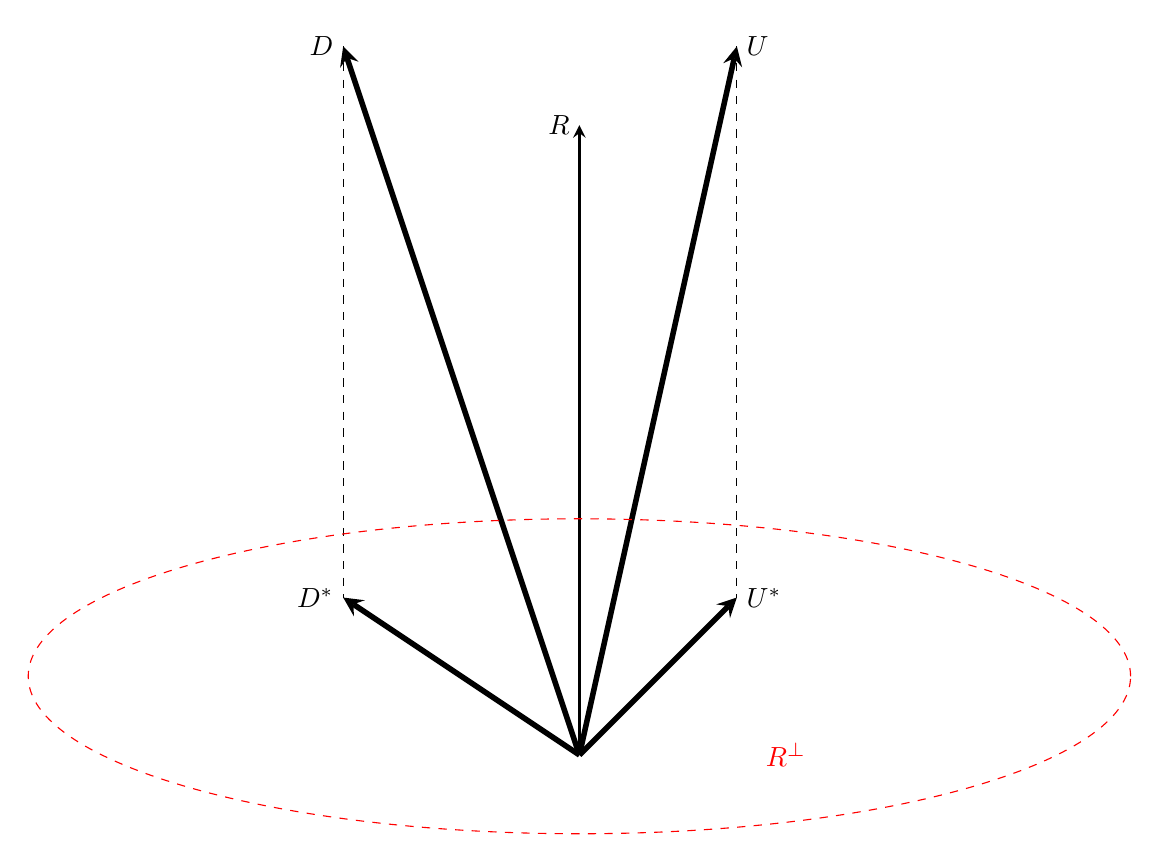
\begin{tikzpicture}
    \coordinate [label=right:$U$] (U) at (2,9);
    \coordinate [label=right:$U^*$] (Ustar) at (2,2);
    \coordinate [label=left:$D$] (D) at (-3,9);
    \coordinate [label=left:$D^*$] (Dstar) at (-3,2);
    \coordinate [label=left:$R$] (R) at (0,8);
    \coordinate (0) at (0,0);
    \coordinate [label=left:$\color{red} R^{\perp}$] (Rort) at (3, 0);


    \draw[line width=2pt,-stealth] (0)--(U);
    \draw[line width=2pt,-stealth] (0)--(D);
    \draw[line width=2pt,-stealth] (0)--(Ustar);
    \draw[line width=2pt,-stealth] (0)--(Dstar);
    \draw[line width=1pt,-stealth] (0)--(R);
    \draw[dashed] (U)--(Ustar);
    \draw[dashed] (D)--(Dstar);
    \draw[dashed, red] (0,1) ellipse (7 and 2);
   
   
  \end{tikzpicture}
\end{center}
\[
\cos \measuredangle{UD} = \Corr(U, D), \quad \cos \measuredangle{U^*D^*} = \pCorr(U, D; R)
\]

\end{frame}


\begin{frame}
  \frametitle{PACF}

  \begin{block}{Определение}
    Для стационарного процесса $(y_t)$ функцию 
    \[
      \varphi_{kk} = \pCorr(y_t, y_{t+k}; y_{t+1}, \ldots, y_{t+k-1}).
    \] 
    называют \alert{частной автокорреляционной}. 
  \end{block}
\end{frame}

\begin{frame}
  \frametitle{ACF и PACF: интуиция}

  Для \alert{стационарного процесса}!

  \begin{itemize}
    \item ACF:
    \[
      \rho_k = \Corr(y_t, y_{t+k}).
    \]
    \alert{Общая сила} связи $y_t$ и $y_{t+k}$.
    \item PACF:
    \[
      \varphi_{kk} = \pCorr(y_t, y_{t+k}; y_{t+1}, \ldots, y_{t+k-1}).
    \]
    \alert{Сила} связи $y_t$ и $y_{t+k}$ при \alert{разорванных} связях через промежуточные наблюдения.
  \end{itemize}
\end{frame}

\begin{frame}
  \frametitle{Почему двойной индекс?}

  \[
  \varphi_{33} = \pCorr(y_t, y_{t+3}; y_{t+1}, y_{t+2}).  
  \]
  \pause
  \[
  \varphi_{23} = \pCorr(y_t, y_{t+2}; y_{t+1}, y_{t+3}).  
  \]
  \pause
  \[
  \varphi_{13} = \pCorr(y_t, y_{t+1}; y_{t+2}, y_{t+3}).  
  \]
\end{frame}

\begin{frame}
  \frametitle{Выборочная PACF через остатки}

  \begin{block}{Корреляция остатков}
    $PACF_4$ — выборочная корреляция \alert{между остатками} $a_t$ и остатками $b_t$.

    $a_t$ — остатки из регрессии
    \[
      y_t \text{ на } 1, y_{t-1}, y_{t-2}, y_{t-3}.
    \]

    $b_t$ — остатки из регрессии
    \[
      y_{t-4} \text{ на } 1, y_{t-1}, y_{t-2}, y_{t-3}.
    \]
  \end{block}
\end{frame}


\begin{frame}
  \frametitle{Выборочная PACF через коэффициент}

  \begin{block}{Оценка коэффициента}
    $PACF_4$ — оценка \alert{последнего коэффициента} в множественной регрессии:
      \[
        \hat y_t = \hat\beta + \hat\beta_1 y_{t-1} + \ldots + \hat\beta_4 y_{t-4}, \quad PACF_4 = \hat\beta_4.
      \]
  \end{block}

\end{frame}

\begin{frame}
  \frametitle{Выборочная и истинная PACF}
  \begin{itemize}[<+->]
    \item Истинная PACF есть \alert{только у стационарного} процесса. 
    \item Выборочную PACF можно посчитать \alert{у любого} процесса. 
    \item По выборочной PACF иногда \alert{можно судить} о стационарности. 
    \item Оба способа дают состоятельные оценки для стационарного процесса. 
    \item Способ с выборочной корреляцией остатков гарантирует числа из отрезка $[-1;1]$.
  \end{itemize}

\end{frame}

\begin{frame}{Частная корреляция: итоги}

  \begin{itemize}[<+->]
    \item Ковариация задаёт геометрию. 
    \item Частная корреляция — корреляция \alert{очищенных} величин.
    \item Во временных рядах очищаем два наблюдения от \alert{промежуточных}.
    \item Оцениваем частную корреляцию.
  \end{itemize}
\end{frame}



